\section{Information flows in the DGA}
\label{sec:dga_flows}

In this Section, a detailed description of the DGA and its core legislative objectives is provided, including the introduction of use cases where Semantic Web technologies and decentralised data environments can be leveraged to aid data intermediaries and data altruism organisations to implement their services while fulfilling their renewed legal duties, in particular, related to the reporting of their activities and how they use personal and non-personal data from data subjects and data holders, respectively.

In February 2020, the~\cite{european_commission_communication_2020} introduced a series of regulatory proposals aimed at legislating the European strategy for data, encompassing a set of new regulatory proposals aimed at governing the utilisation of non-personal and public data, regulating digital services and markets, and fostering the creation of common European data spaces.
By prioritising data and ensuring its accessibility across sectors, this transformation must also maintain the interests of both data subjects and data holders, while supporting trusted entities to facilitate data sharing aligned with new regulations.
Among these proposals was the Data Governance Act~\citeyearpar{noauthor_regulation_2022}, a regulation presented to enhance data accessibility and foster trust in data intermediation services throughout the EU.
Following approval by both the European Parliament and the European Council, this legislation entered into force on 23 June 2022 and, following a 15 month grace period, has been applicable since September 2023.
Similarly to other data-related legislation within the EU, the DGA relays new rights and obligations to entities holding both personal and non-personal data.
It also regulates the operations of data users and two categories of data-related services related to data intermediation and altruism.
The principal objectives of this legislation include:

\begin{enumerate}
    \item[(i)] Facilitating the reuse of protected public-sector data while maintaining its privacy and confidentiality, particularly in cases where such data is subject to the rights of others, including trade secrets, personal data protection, and data safeguarded by intellectual property rights.
    \item[(ii)] Regulating and maintaining a register of data intermediation service providers, which facilitate data sharing among enterprises and support individuals to have a `personal data-sharing intermediary', designed to aid them in exercising their rights, e.g., under the GDPR.
    \item[(iii)] Allowing businesses and data subjects to voluntarily contribute data for altruistic purposes, such as medical research.
    \item[(iv)] Establishing a novel supervisory authority, the European Data Innovation Board (EDIB), tasked with supervising the operations of data intermediation service providers and data altruism organisations.
    This Board comprises representatives from regulatory bodies overseeing data intermediation and altruism activities across all EU member states, from the EDPB and EDPS, from the European Union Agency for Cybersecurity (ENISA) and the European Commission, as well as experts in standardisation, portability, interoperability, and other pertinent stakeholders.
\end{enumerate}

The main hurdles to overcome in order to achieve these objectives are associated with:

\begin{enumerate}
    \item[(i)] \textit{Availability/Discovery of datasets}: in the absence of technical assistance for creating data spaces and reliable data-sharing platforms, individuals and organisations will not have tools to share their data for the common good, nor will they have adequate support to exercise their data-related rights. On the other hand, data users lack the necessary tools to search for the data they require.
    \item[(ii)] \textit{Establishment of data access and usage conditions}: with the unavailability of standards and metadata vocabularies to articulate machine-readable policies, setting conditions for the usage and access to personal, non-personal, and public-sector data -- rooted not just in legal frameworks but also in ethical, organisational, and social norms -- will lead to interoperability challenges among entities providing and seeking data access.
    \item[(iii)] \textit{Reporting duties}: without maintaining structured records of their activities, providers of data intermediation services and organisations engaged in data altruism will depend on manual methodologies to generate documentation reporting their accountable and responsible data-handling practices.
\end{enumerate}

Thus, to tackle the challenges at hand, the first task defined in this Thesis is related to the identification of relevant flows of information between DGA-regulated entities, as well as what specific information items need to be shared or kept by which entities.
Since the DGA both advocates for data availability and legislates data sharing, a delineation of information flows among data-sharing entities can be specified.
In addition, as a result of these interactions, certain registers and records of activities must be maintained for transparency and accountability, in line with previous EU data protection law, e.g., the GDPR.
Figure~\ref{fig:dga_flow} outlines the entities and their corresponding information flows identified within this context.
Their respective definitions are outlined below.

\begin{figure}[ht]
\centering
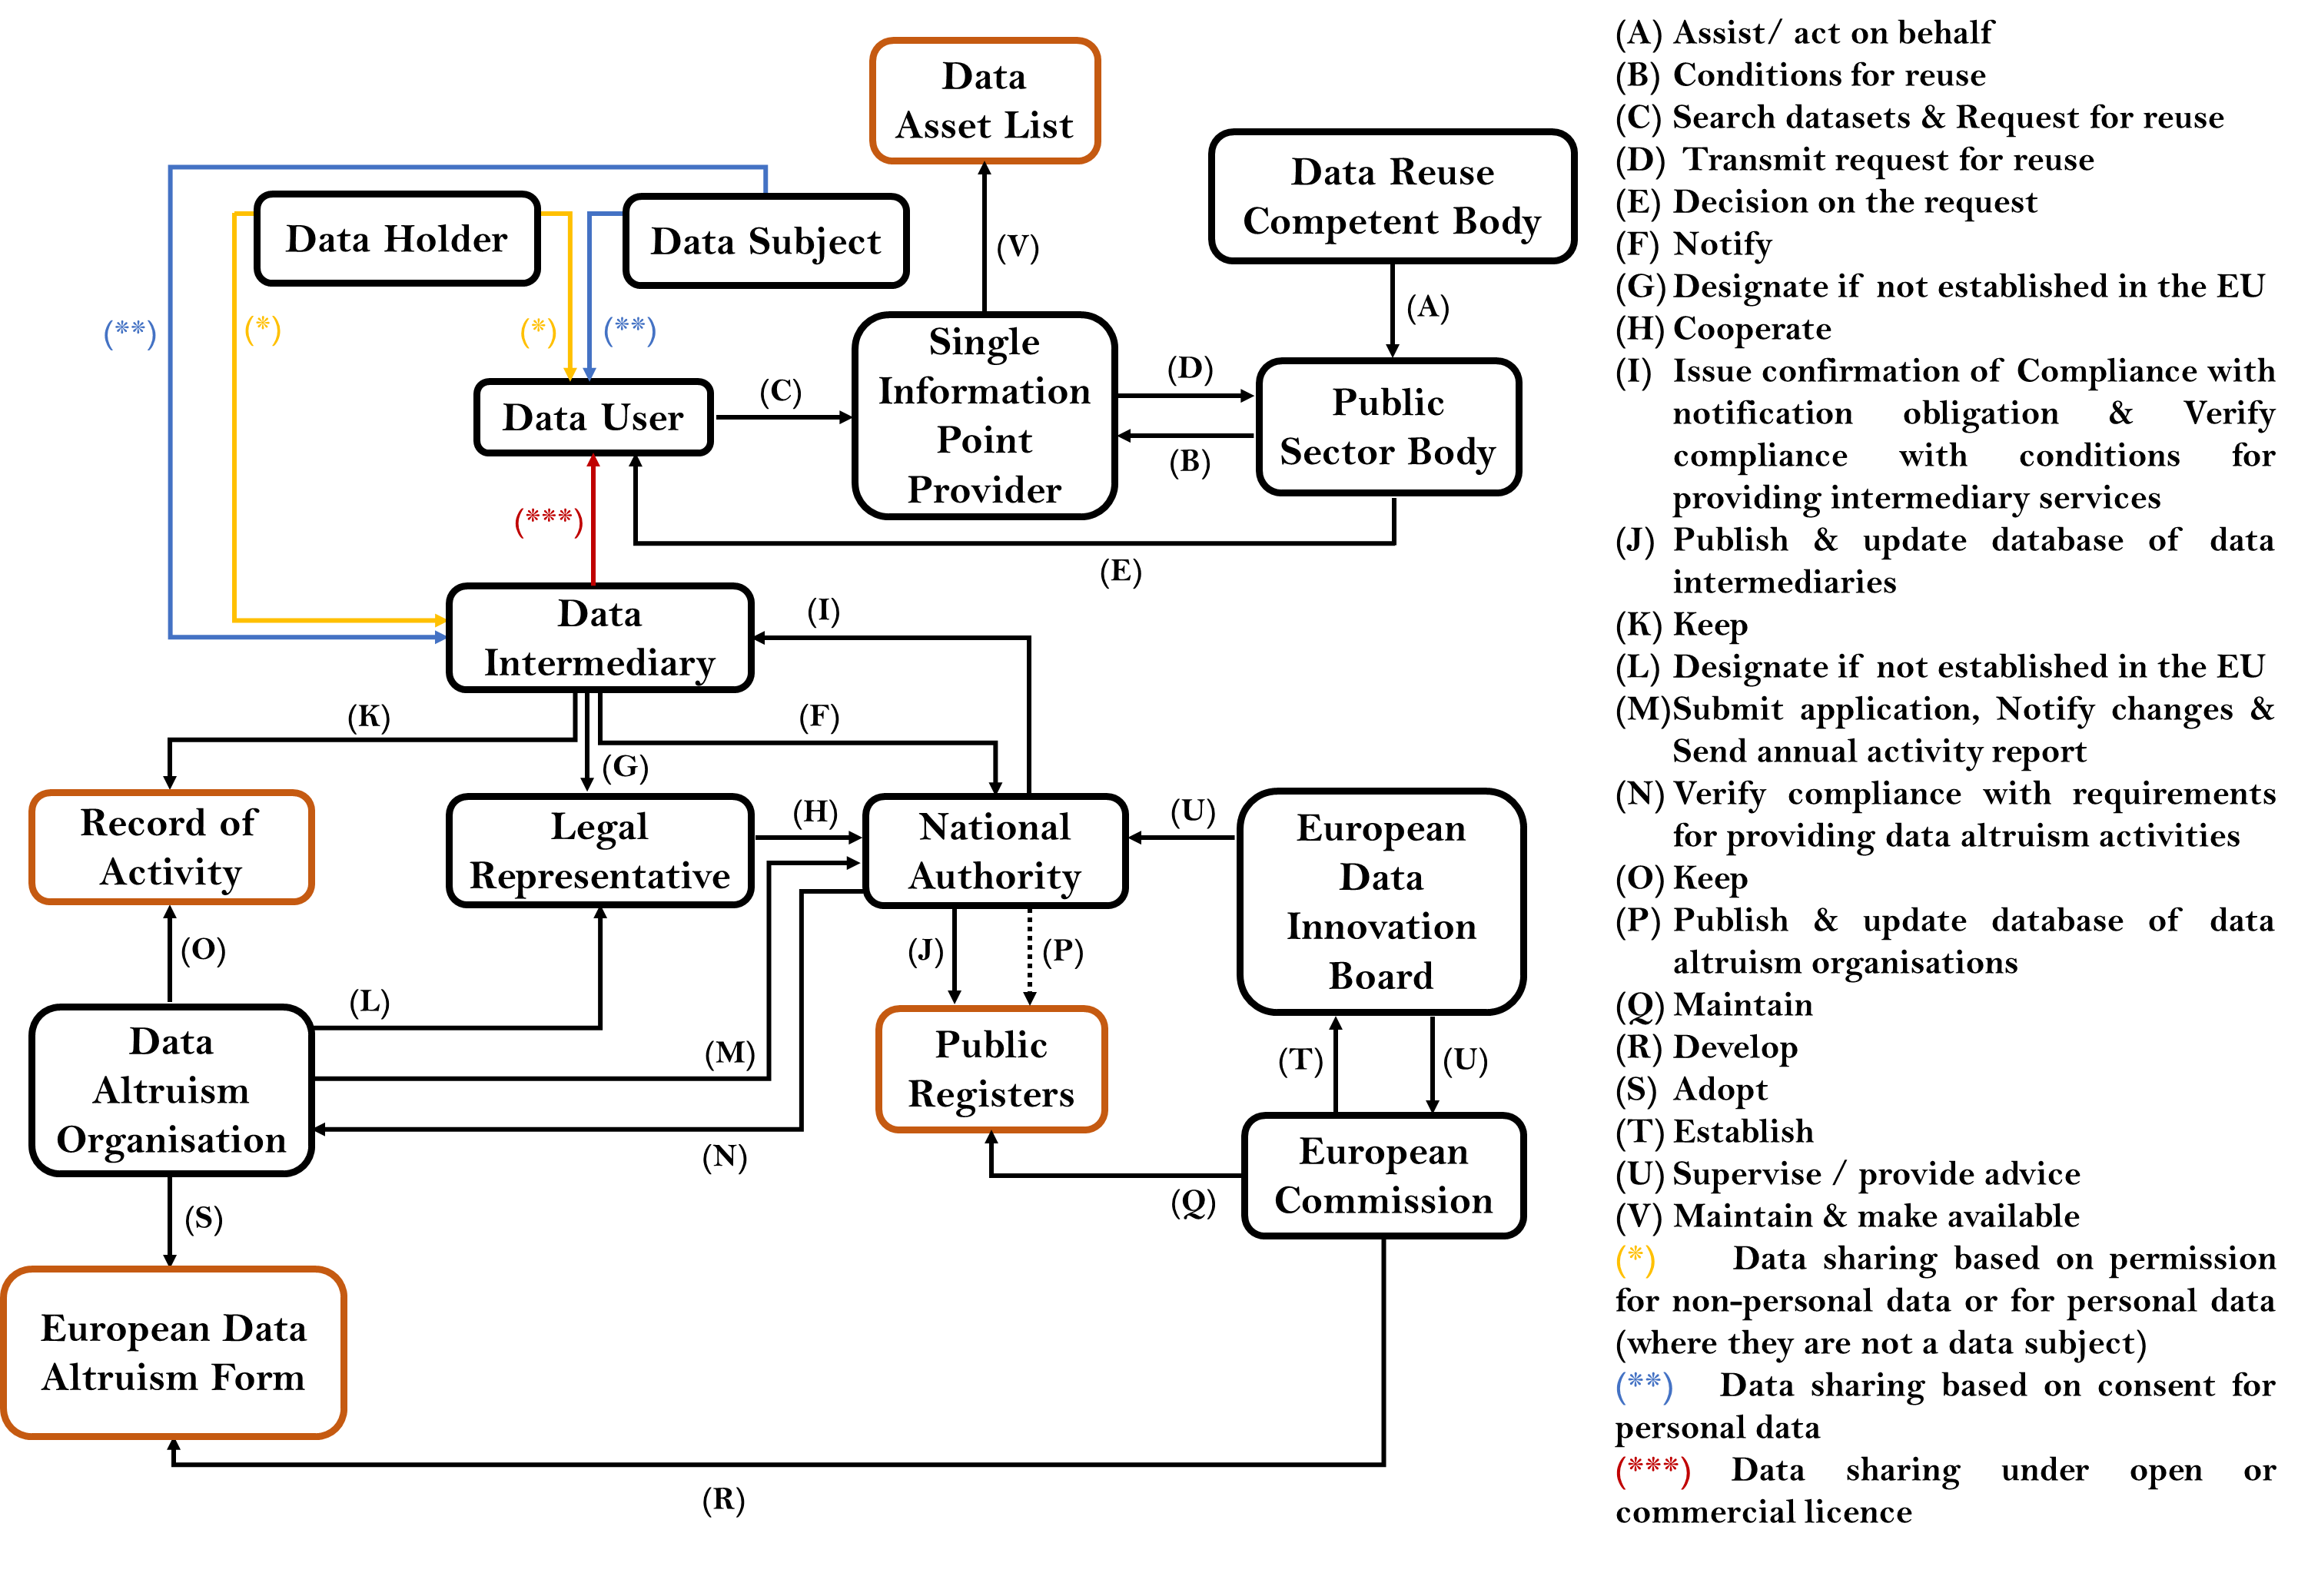
\includegraphics[width=\textwidth]{figures/chapter-7/information-flows.png}
\caption[Flows of information between DGA entities.]{Flows of information between DGA entities, adapted from~\cite{esteves_semantics_2023}. The concepts in a black box are the entities and the ones in an orange box are the legal documentation that needs to be created and maintained by said entities. The direction of the arrows represents the direction of the information flow between entities. A short description of each flow is specified on the right side of the Figure.}
\label{fig:dga_flow}
\end{figure}

\textbf{Data Subject} Natural person whose personal data is undergoing any kind of processing (as defined in the GDPR).

\textbf{Data Holder} An entity that can share personal and/or non-personal data.

\textbf{Data User} An entity that wishes to use personal and/or non-personal data for commercial or non-commercial purposes.

\textbf{Data Intermediation Service Provider} An entity that establishes commercial relationships for the sharing of data among data subjects, data holders, and data users.

\textbf{Data Altruism Organisation} An not-for-profit organisation that collects and shares data for altruistic purposes.

\textbf{Public Sector Body} An entity or group of entities governed by public law from one or more State, regional and/or local authorities.

\textbf{Legal Representative} A legal entity's representative appointed to act on behalf of a data intermediation service provider or altruistic organisation.

\textbf{Competent Body} An entity appointed by a public sector body to offer legal and technical assistance regarding the access and reuse of public sector data.

\textbf{Single Information Point Provider} An entity tasked with receiving and forwarding requests for public data reuse.

\textbf{Competent Authorities} Authorities in charge of supervising the activity of data intermediation service providers and data altruism organisations and maintaining a public register of said entities.

\textbf{European Data Innovation Board} A supranational authority responsible for supervising the operations of data intermediaries and data altruism organisations.

As illustrated in Figure~\ref{fig:dga_flow} by a red arrow, the data intermediation service provider, or data intermediary, provides data users with access to data under open or commercial license conditions and, as illustrated with the (K) arrow, must maintain a record of its activities.
This diagram was crafted from an analysis of DGA's Chapters II (`Re-use of certain categories of protected data held by public sector bodies'), III (`Requirements applicable to data intermediation services'), IV (`Data altruism'), and VI (`European Data Innovation Board')~\citeyearpar{noauthor_regulation_2022}.
Each article within these chapters was meticulously examined to identify interactions among the identified entities.
Whenever an information flow was identified between multiple entities, the respective interaction was documented in the diagram.
Furthermore, requirements related to compliance documentation are also included in the diagram.
These requirements entail the recording of information that can be automated using semantic technologies.

In the following three Sections, the information flows concerning the conditions for reusing public data (Section~\ref{sec:reuse}), the maintenance of registers of altruistic and intermediary entities and respective activities logs (Section~\ref{sec:registers}), and the forms to record data altruism terms (Section~\ref{sec:altruism}) are described in detail.
These areas highlight the strengths of using semantic technologies to effectively aid the previously mentioned entities in automating their DGA compliance tasks.
For each example use case, a systematic analysis of the pertinent information flows and the corresponding data exchange requirements was conducted manually.
The findings are organised and presented in the subsequent Sections.

\subsection{Conditions for the reuse of data held by public sector bodies}
\label{sec:reuse}

DGA's Chapter II legislates the reuse of data stored by public sector bodies, encompassing the specification of which data categories are regulated (Article 3~\citeyearpar{noauthor_regulation_2022}), the conditions required from public sector bodies to provide such services (Articles 5 and 6~\citeyearpar{noauthor_regulation_2022}), and the delineation of single information point providers and their role in facilitating data users' search for and request of datasets for reuse purposes (Articles 8 and 9~\citeyearpar{noauthor_regulation_2022}).
To keep such data, these entities need to have in place safeguards to protect their commercial and statistical confidentiality, intellectual property rights of third parties, and personal data-related rights.
Moreover, they have to publish the dataset reuse conditions, and the respective data request procedure, in a transparent and publicly accessible manner.
The reuse must be contracted, with a maximum duration of one year, including the categories of data being used as well as the purpose for the reuse. 
Public sector bodies also have the right to obtain guidance and technical support from a competent body, which must be appointed by each EU member state.
These appointed entities are responsible for providing guidance on data formats and storage, assisting in the implementation of privacy-preserving methods to protect personal data integrity, and supporting activities to obtain consent from data subjects and permission from data holders.

A complete list of information required from public sector bodies, along with a reference to the pertinent articles in the DGA, is summarised in Table~\ref{tab:conditions_public_data}.
This information, which may be further specified with the aid of a competent body (as previously mentioned and indicated by the (A) arrow in Figure~\ref{fig:dga_flow}), should be communicated to the single information point provider (as depicted by the (B) arrow).
This enables data users to search for datasets ((C) arrow) and submit reuse requests through the single information point ((D) arrow). 
Additionally, single information point providers are obligated to maintain and disclose a data asset list (illustrated by the (V) arrow), comprising details on available resources and their reuse conditions.

\begin{table}[ht]
\centering
\caption{Information items about public sector bodies' services.}
\label{tab:conditions_public_data}
\begin{tabular}{c||l}
\textbf{Article} & \multicolumn{1}{l}{\textbf{Information items}}\\ \hline\hline
2.9 & Data user/categories of users \\ \hline
5.1 & Public sector body information \\ \hline
5.1 & Competent body information \\ \hline
5.2 & Categories of data \\ \hline
5.2 & Purposes for usage and access \\ \hline
5.2, 5.3(a) & Nature of data \\ \hline
5.3(b), 5.3(c) & Processing environment \\ \hline
5.5 & Measures to prevent re-identification of data holders/subjects \\ \hline
5.9 & Third party recipients \\ \hline
6.2 & Fees \\ \hline
8.2 & Data format \\ \hline
8.2 & Data size \\ \hline
9 & Procedure to request reuse
\end{tabular}
\end{table}

\subsection{Registers and records of altruistic and intermediation entities}
\label{sec:registers}

DGA is also the first of its kind to regulate the activity of data intermediation service providers and altruistic organisations, with the requirements being outlined in Chapters III and IV.
Regarding data intermediation, such entities \textit{``aim[s] to establish commercial relationships for the purposes of data sharing between an undetermined number of data subjects and data holders on the one hand and data users on the other, through technical, legal or other means''}~\citeyearpar{noauthor_regulation_2022}.
Moreover, as defined in Article 11~\citeyearpar{noauthor_regulation_2022}, entities wishing to provide data intermediation services must notify their competent national authority of their intentions (indicated by the (F) arrow in Figure~\ref{fig:dga_flow}).
Subsequently, the national authority is mandated to publish and maintain an updated public register of intermediaries (represented by the (J) arrow) and oversee their activities ((I) arrow).
Article 12~\citeyearpar{noauthor_regulation_2022} includes a list of conditions for the provision of this service, e.g., providers should have tools to convert data into specific formats, use standards to promote interoperability across sectors, gather data subjects' consent and data holders' permission terms, as well as update or withdraw these terms, maintain records of their activity, and appoint a legal representative if the data intermediation entity is not established in the EU (shown by the (G) arrow).
Furthermore, the data intermediation service provider must maintain a log record of its activities (indicated by the (K) arrow).
This log must include entity-related information available in the public register of intermediation providers, such as name, public website, legal status, ownership structure, subsidiaries, registration number, address, and details regarding the provided service type.
A detailed list of the information used to notify authorities regarding the start of activity of a data intermediation service provider and the conditions to provide such service are available in Table~\ref{tab:registers_intermediation}.

\begin{table}[htp]
\centering
\caption[Information items related to the activity of data intermediation service providers.]{Information used to notify authorities regarding the start of activity of a data intermediation service provider and the conditions to provide such service, which need to be kept in a record of activities. Information items marked with (*) are kept in the public register of data intermediaries.}
\label{tab:registers_intermediation}
\begin{tabular}{c||l}
\textbf{Article} & \textbf{Information items} \\ \hline\hline
11.3 & Legal representative if not established in the EU (*) \\ \hline
11.6(a) & Name of the data intermediation services provider (*) \\ \hline
11.6(b) & Data intermediation services provider’s legal status (*) \\ \hline
11.6(b) & Data intermediation services provider’s form (*) \\ \hline
11.6(b) & Data intermediation services provider’s ownership structure (*) \\ \hline
11.6(b) & Data intermediation services provider’s relevant subsidiaries (*) \\ \hline
11.6(b) & Data intermediation services provider’s registration number (*) \\ \hline
11.6(c) & Address of the data intermediation services provider (*) \\ \hline
11.6(c) & \begin{tabular}[c]{@{}l@{}}Address of the representative of the data intermediation\\services provider (*)\end{tabular} \\ \hline
11.6.(d) & Public website (*) \\ \hline
11.6(e) & Data intermediation services provider’s contact persons \\ \hline
11.6(e) & Data intermediation services provider’s contact details \\ \hline
11.6(f) & Description of the data intermediation service (*) \\ \hline
11.6(f) & Type of data intermediation service (*) \\ \hline
11.6(g) & Estimated date for starting the activity (*) \\ \hline
11.6(g) & Date of the notification (*) \\ \hline\hline
\textbf{Article} & \textbf{Conditions to provide intermediation services} \\ \hline\hline
12(b) & Pricing \\ \hline
12(c) & Date and time of creation of data \\ \hline
12(c) & Geolocation data \\ \hline
12(c) & Duration of the activity \\ \hline
12(c) & \begin{tabular}[c]{@{}l@{}}Connections to other natural or legal persons established by the\\person who uses the data intermediation service\end{tabular} \\ \hline
12(d) & Data format \\ \hline
12(d) & Convert the data into specific formats \\ \hline
12(e) & Tools to facilitate the exchange of data \\ \hline
12(f) & Terms of service \\ \hline
12(g,h,i,j,l) & \begin{tabular}[c]{@{}l@{}}Technical and organisational measures to protect, provision and\\ensure interoperability of data\end{tabular} \\ \hline
12(k) & \begin{tabular}[c]{@{}l@{}}Notification of unauthorised transfer, access or use of the\\non-personal data\end{tabular} \\ \hline
12(m) & Tools to facilitate exercising of data subjects' rights \\ \hline
12(n) & Third country jurisdiction \\ \hline
12(n) & Tools to obtain/withdraw consent/permission \\ \hline
12(o) & Log record of the data intermediation activity
\end{tabular}
\end{table}

For entities aiming to establish themselves as data altruism organisations, as outlined in DGA's Article 19~\citeyearpar{noauthor_regulation_2022}, the process entails submitting an application to their competent national authority (which may be the same authority regulating national data intermediation service providers for instance) to express their intentions (illustrated by the (M) arrow in Figure~\ref{fig:dga_flow}).
Upon approval, the national authority is required to include information about the organisation in a public register of data altruism organisations (depicted by the (P) arrow).
This register encompasses details such as the organisation's name, public website, legal status, form, registration number, contact information for the entity and its representative (if applicable), as well as information regarding the altruistic purposes underlying the organisation's activities.
Furthermore, the organisation must publish and regularly update a uniform and structured record of its data altruism activities ((O) arrow).
This record is submitted annually to the national authority for compliance verification (indicated by the (M) and (N) arrows).
It must document the organisation's data altruism activities, including the nature and categories of data it handles.
Additionally, it should contain logs of data users, their contact details, the processing date and duration, the altruistic purposes for data usage, fees paid by users or other sources of income, used technical processing means, and a summary of processing results.
A detailed list of the information used to notify authorities regarding the start of activity of a data altruism organisation and the mandatory information items that need to be kept in the record of data altruism activity are available in Table~\ref{tab:registers_altruism}.

\begin{table}[htp]
\centering
\caption[Information items related to the activity of data altruism organisations.]{Information used to open activity as a data altruism organisation and respective information items that need to be kept in the record of said activity. Information items marked with (*) are kept in the public register of data altruism organisations.}
\label{tab:registers_altruism}
\begin{tabular}{c||l}
\textbf{Article} & \textbf{Information items} \\ \hline\hline
19.3 & Legal representative if not established in the EU (*) \\ \hline
19.4(a) & Name of the entity (*) \\ \hline
19.4(b) & Entity’s legal status (*) \\ \hline
19.4(b) & Entity’s form (*) \\ \hline
19.4(b) & Entity’s registration number (*) \\ \hline
19.4(c) & Statutes of the entity \\ \hline
19.4(d) & Entity’s sources of income \\ \hline
19.4(e) & Address of the entity \\ \hline
19.4(e) & Address of the representative of the entity \\ \hline
19.4(f) & Public website (*) \\ \hline
19.4(g) & Entity’s contact persons (*) \\ \hline
19.4(g) & Entity’s contact details (*) \\ \hline
19.4(h) & Altruistic purposes (*) \\ \hline
19.4(i) & Nature of data \\ \hline
19.4(i) & Categories of personal data \\ \hline\hline
\multicolumn{1}{c||}{\textbf{Article}} & \textbf{Records of Altruism Activity} \\ \hline\hline
20.1(a), 20.2(c) & Data users \\ \hline
20.1(a) & Data users' contact details \\ \hline
20.1(b) & Date of the processing of data \\ \hline
20.1(b) & Duration of the processing of data \\ \hline
20.1(c), 20.2(c) & Altruistic purpose for processing \\ \hline
20.1(d) & Fees paid by data users \\ \hline
20.2(a) & Information on its activities \\ \hline
20.2(b) & Description of the objectives of general interest \\ \hline
20.2(c) & Technical means used for processing \\ \hline
20.2(d) & Summary of the results of the data processing \\ \hline
20.2(e) & Sources of revenue
\end{tabular}
\end{table}

\subsection{Data altruism forms}
\label{sec:altruism}

Data altruism as a term was first introduced by the DGA.
This term relates to the sharing of personal and non-personal data, based on data subjects' consent and data holders' permission, for the `common good'.
This entails purposes such as improving healthcare, combating climate change, or performing scientific research.
Moreover, the proposed visions for a European Health Data Space~\citeyearpar{noauthor_proposal_2022} and the Data Act~\citeyearpar{noauthor_dataact_2022} also emphasise the altruistic reuse of data, with the Health Data Spaces proposal, in particular, focusing on the challenges brought on by the access and sharing of electronic health data for scientific research and public interest purposes.
In this context, each EU member state can establish its altruism policy and has to appoint a competent authority to oversee the activity of altruistic organisations (it can be the same as the one that supervises intermediation providers).
As mentioned in the previously Section, said authority also has to keep up-to-date, public registers of altruistic organisations, and organisations themselves have to maintain records of their activities, in particular, to produce annual reports to share with the relevant competent authority.
To facilitate this activity, a European data altruism consent form will be facilitated by the EC to \textit{``allow the collection of consent or permission across Member States in a uniform format''}, as described in Article 25~\citeyearpar{noauthor_regulation_2022} and indicated by the (R) arrow in Figure~\ref{fig:dga_flow}.
The development of this form involves consultation with GDPR's overseeing body, the EDPB, the forthcoming EDIB, and other relevant stakeholders.
Once developed, it is to be adopted by data altruism organisations (depicted by the (S) arrow) to document both the consent provided by data subjects to share their personal data and the permissions granted by data holders to share their non-personal data.
Furthermore, these forms are required to be maintained in both human and machine-readable formats.

% Comparison with GDPR flows